\chapter{Procesamiento de Imágenes Digitales}

\section{Que es la Visión Artificial?}
El objetivo de la visión artificial es utilizar cámaras para analizar o entender escenas del mundo real. Es una disciplina que estudia problemas metodológicos y algorítmicos, además de la implementación de soluciones diseñadas \parencite{Klette2014-oo}.
La visión artificial nos permite saber si un auto se encuentra en su carril, cuantas personas se encuentran en un lugar, cual es la distancia desde una cámara a un edificio y, reconocer una persona específica; basado en imágenes o video.
Recientemente ha habido un avance sólido en la visión artificial, con lo que las áreas de aplicación han aumentado. En productos modernos, se utiliza en aplicaciones para teléfonos inteligentes, asistencia para conductores de vehiculos, vehiculos auto-manejados (self-driving cars), o en la interacción usuario-videojuego.  Por otro lado, en la automatización industrial, se utiliza para el control de calidad o de proceso y, en la industria del cine, para la creación de avatares y mundos basados en imágenes o video, entre otros.  Estos son unos cuantos ejemplos de áreas en las que se satisface una necesidad de procesar información almacenada en imágenes o video. 


\section{Características de un Sistema de Visión}
Un sistema de visión evalúa los datos que se encuentran en una imagen (originados de una cámara), extrae y procesa los datos y luego ejecuta una acción con los resultados.

Por ejemplo, un dispositivo de control de parqueo. Este sistema observa un espacio de parqueo y detecta violaciones de parqueo en las que vehículos no autorizados intentan parquear en el espacio. Si fuese, en cambio, un vehículo autorizado o si el espacio estuviese desocupado, no hubiese ninguna violación. A pesar de ser conceptualmente simple, el problema presenta complejidades:

\begin{itemize}
    \item Las condiciones de luz afectan la detección de color y la distinción del vehículo del fondo.
    \item La ligera variación del lugar de parqueo del vehículo puede dificultar la detección del vehículo contra un espacio desocupado. 
    \item El vehículo puede estar sucio, dificultando la detección de un vehículo autorizado o de un vehículo no autorizado. 
    \item El lugar de parqueo puede estar cubierto de nieve, dificultando saber si el espacio se encuentra desocupado.
\end{itemize}
Para encarar las complejidades mencionadas, un sistema de visión usualmente realiza dos tareas: filtrar la entrada para reducir el rango de información a procesar y, extraer las características relevantes de la(s) imágen(es) \parencite{Demaagd2012-qb}.

\section{Imagen Digital}
Una imagen digital puede considerarse como una representación discreta de información, que posee tanto datos espaciales y de intensidad (color) \parencite{Solomon2011-xz}.
Mientras que una imagen es una representación bidimensional de una escena tridimensional, una imagen digital es básicamente una representación numérica de una imagen. Los diferentes sistemas de procesamiento de imágenes incluyen la adquisición de imágenes, su almacenamiento, procesamiento y exposición \parencite{Jayaraman2011-jb}.
\section{Adquisición de la Imagen}
La adquisición de la imagen digital es el primer proceso que cumple un sistema de reconocimiento de matrículas. Existen múltiples maneras de adquirir imágenes, y uno de ellos es a traves de Cámaras IP (IPC); para estas cámaras, existen múltiples fabricantes y cada uno puede adoptar un protocolo propietario. En este sentido, se propone un diseño de un software de control vehicular compatible con la especificación ONVIF. La especificación ONVIF define un protocolo común para el intercambio de información a través de dispositivos basados en IP. 

\subsection{Especificación ONVIF}
El Open Network Video Interface Forum \parencite{Onvif2016-bt}. fue fundado por Axis Communications, Bosch Security Systems y Sony Corporation Actualmente cuenta con 455 socios: 41 socios completos, 20 socios contribuyentes, 369 socios usuarios y 25 socios observadores. La especificación incluye descubrimiento automatizado de  dispositivos,  además de  transmisión de vídeo y metadatos. ONVIF hace uso de servicios web y provee una conformidad formal para los procesos. En este sentido, asegura la interoperabilidad entre dispositivos, sin importar la marca. 


\subsubsection{Comunicación}
El especificación ONVIF define una capa de red de dispositivos de seguridad IP, descrita por servicios web basados en los definidos por la Organización para el Avance de Estándares de Información Estructurada (OASIS). La definición de un cliente está provista en WSDL (Web Service Description Language) para asegurar la integración de productos sin importar la marca de los mismos. Las estructuras de datos y su intercambio entre servicios web proveedores y solicitantes se basa en el protocolo Simple Object Access Protocol (SOAP). SOAP es un protocolo de intercambio de mensajes que puede ser implementado a través de HTTP, HTTPS, RTSP, etc. \parencite{Onvif2016-dc}.

    \begin{figure}[H]
        \centering
        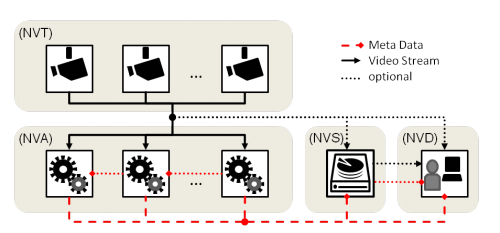
\includegraphics[width=0.80\textwidth]{onvif-arch}
        \caption{Arquitectura de una red basada en ONVIF \parencite{Senst2011-bb}}
        \label{fig:onvif-arch}
    \end{figure}
    
Cada dispositivo integrado en una red conforme al protocolo ONVIF debe implementa un servicio que es categorizado en cuatro clases:

\begin{itemize}
\item \textbf{Transmisor de Vídeo en Red (NVT):} provee uno o más flujos de vídeo, como una cámara o una caja que combina los flujos de vídeo de múltiples cámaras.
\item \textbf{Análisis de Vídeo en Red (NVA):} son dispositivos utilizados para analizar vídeo, audio o metadatos y proveen información adicional que no es entregada con el flujo de vídeo. 
\item \textbf{Exposición de Vídeo en Red (NVD): }provee la representación del flujo de vídeo y la interfaz entre el sistema y los operadores humanos.
\item \textbf{Almacenamiento de Vídeo en Red (NVS):} provee los medios para grabar multimedia transmitida y metadatos, además de la capacidad de acceder a estos datos de una manera estructurada.
\end{itemize}

De acuerdo con la especificación ONVIF, las funcionalidades de análisis que proporcionan los sistemas de seguridad de vídeo pueden considerarse NVAs \parencite{Senst2011-bb}.

\section{Extracción de Características de una Imagen}

Los valores numéricos que representan a una imagen son llamados Descriptores o Características, ya que expresan información acerca de la imagen. Los descriptores son utilizados para extraer de las imágenes información útil para un usuario. Según la información de la que se está hablando, se los puede dividir en distintos grupos como: descriptores de colores, texturas o formas. \parencite{Deselaers2008-zg}.

Los descriptores comúnmente utilizados en el análisis de matrículas incluyen descriptores de forma, simetría \parencite{Kim2001-yv}, proporción de altura y ancho \parencite{Naito2000-im}, color \parencite{Kim1996-js}, variación de valores de intensidad \parencite{Draghici1997-gz}, etc.. Por otro lado, los descriptores de caracteres incluyen: línea \parencite{Yu2000-tm}, masas amorfas (blobs) \parencite{Hontani2001-lk}, relación de aspecto de los caracteres \parencite{Hermida1997-ds}, distribución de intervalos entre caracteres \parencite{Poon1995-pw} y el alineamiento de los mismos \parencite{Soh1994-mc}. En la práctica, un pequeño conjunto de descriptores de un objeto que sean robustos, confiables y fáciles de detectar son suficientes para describir al mismo \parencite{Chang2004-kg}. 

En el análisis de imágenes se extrae descriptores (información relevante de las imágenes) a través de técnicas de procesamiento de imágenes digitales para realizar posteriormente el reconocimiento y clasificación de los mismos. Las tareas de análisis de imágenes pueden ser tan simples como leer un código de barras como identificar una persona por su rostro. \parencite{Solomon2011-xz}


\section{Segmentación de Imágenes Digitales}

La segmentación de imágenes es esencial para el procesamiento de imágenes al ser el primer paso antes de realizar la extracción, clasificación, descripción de características; consiste en subdividir la imagen en base a sus regiones u objetos que la constituyen. Es uno de los procesos más difíciles en el diseño de sistemas de visión artificial y se mantiene como un campo activo de la investigación de técnicas de procesamiento de imágenes y visión artificial \parencite{Solomon2011-xz}.

Luego de haber realizado una segmentación, se distingue un primer plano y un plano de fondo. Una segmentación correcta depende estrictamente de los tipos de objetos o regiones de interés para la identificación y, se puede realizar a través de dos maneras:
\begin{itemize}
\item \textbf{Métodos basados en bordes:} se buscan bordes entre regiones entonces la clave es identificar marcadas diferencias entre un grupo de píxeles
\item \textbf{Métodos basados en regiones:} Se asignan píxeles a una región según su grado de similitud.
\end{itemize}

\subsection{Uso de Descriptores para la Segmentación}
Con el método más básico de segmentación (umbral de intensidad) la segmentación se realiza utilizando únicamente la intensidad de los píxeles; sin embargo, otros métodos utilizan características y propiedades más sofisticadas de las imágenes para realizar segmentaciones exitosas. En este sentido, existen tres propiedades básicas en las imágenes a la hora de realizar una segmentación:
\begin{itemize}
\item El color permite distinguir entre objetos y fondos. Por ejemplo, segmentar una naranja de un fondo azul.
\item La textura es un concepto no muy bien definido en el procesamiento de imágenes. Se refiere a la variación espacial en la intensidad de una imagen.
\item El movimiento de los objetos en una secuencia de imágenes puede ser útil para la segmentación. 
\end{itemize}
La mayoría de los procesos de segmentación utilizan una o más de las características de color, textura y movimiento de objetos. Existen sin embargo casos en los que es más difícil segmentar objetos: por ejemplo, un avión en movimiento en el cielo no puede distinguirse por su textura usualmente, entonces un análisis de forma podría realizarse. Es importante tener cuidado a la hora de elegir la técnica de segmentación para exitosamente separar al objeto que se busca de su fondo. \parencite{Solomon2011-xz}.

\subsection{Método del Umbral de Intensidad}
El umbral de intensidad es el método más sencillo para la tarea de segmentación. Si se quiere separar objetos en una imagen dada la variación de la intensidad en la imagen, seleccionamos un valor límite de manera que los píxeles cuyo valor sea mayor que el valor límite sean asignados a una región mientras que los que caigan por debajo del valor sean asignados a otra región (adjunta). El umbral de intensidad genera una imagen binaria, como se puede observar en la Figura 10.1.

    \begin{figure}[H]
        \centering
        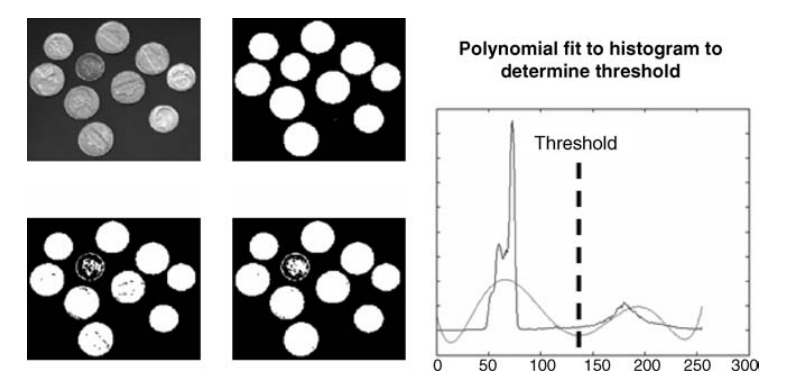
\includegraphics[width=0.80\textwidth]{umbral-intensidad}
        \caption{Figure 10.1 Izquierda superior: imagen original. Derecha Superior: resultado después de realizar una selección manual del umbral de intensidad. Izquierda Inferior: resultado de selección automática del umbral por regresión polinomial al histograma de la imagen. Derecho inferior: resultado de selección automática del umbral por el método de Otsu. La imagen en la derecha muestra el histograma y el resultado de hacer una regresión polinomial de 6to orden \parencite{Solomon2011-xz}}
        \label{fig:umbral-intensidad}
    \end{figure}
    


\section{Clasificación de Características (Detección)}
\subsection{El propósito de la clasificación automática}
La clasificación de células sanas o anormales, separación de frutas de calidad en una planta de empaquetamiento, etc, son ejemplos de clasificación. 

La clasificación sucede en todos los aspectos de la vida y es uno de los primeros pasos necesarios para tomar decisiones. En procesamiento de imágenes, el objetivo de la clasificación es identificar características, patrones o estructuras en una imagen y asignarlos a una clase específica (detección). A pesar de que el ser humano es completamente capaz de realizar tareas de clasificación con bastante precisión, es la única aproximación realista y costo-efectiva la de automatizar la clasificación de grandes volúmenes de datos. Sin embargo, en el momento de hacer esto, la intervención humana es necesaria en dos áreas clave \parencite{Solomon2011-xz}: 

\begin{itemize}
\item \textbf{Especificación de la tarea: }Que se quiere explícitamente que el clasificador logre? Se deben determinar las clases que serán consideradas y que parámetros o variables se consideran importantes para realizar la clasificación. Por ejemplo, a la hora de clasificar células estas se pueden clasificar en normales o anormales, pero un clasificador más complejo que tenga más clases y observe más información y podría también catalogar a los pacientes en categorías como anemia, infección viral, etc.
\item \textbf{Nombramiento de clases: }El proceso de entrenar a un clasificador automático usualmente requiere “nombramiento manual” en las primeras etapas; consiste en asignar ejemplos a clases específicas en base a propiedades seleccionadas y sobresalientes. Esto forma parte del proceso de los llamados “clasificadores supervisados”.
\end{itemize}

\subsection{Clasificación Supervisada y No Supervisada}
Las técnicas de clasificación se pueden agrupar en dos grupos principales: supervisados y no supervisados \parencite{Solomon2011-xz}. 
La clasificación supervisada se apoya en tener datos de entrenamiento en base a los cuales se espera clasificar exitosamente nuevos patrones.
La clasificación no supervisada utiliza técnicas de agrupamiento para clasificar sin información previa el conjunto de características que se observan en una imagen. 

\subsection{Diseño de Módulos de Clasificación }

Los sistemas de clasificación siguen el siguiente diseño, que también puede observarse en la figura \ref{fig:classifier-design}, son: 
\begin{enumerate}
    \item Definición de clases de interés para el problema
\item Exploración de datos, identificando posibles atributos que permitan distinguir óptimamente entre clases
\item Selección y extracción de características que definen el espacio de características discriminatorias entre clases. Por ejemplo, para distinguir entre un leopardo y un león, no es muy preciso distinguir en base a características de forma; en cambio, es más óptimo hacerlo en base a características de color.
\item Construir el clasificador con datos de entrenamiento
\item Probar el clasificador para ver si es necesario ajustar las clases definidas
\end{enumerate}

    \begin{figure}[H]
        \centering
        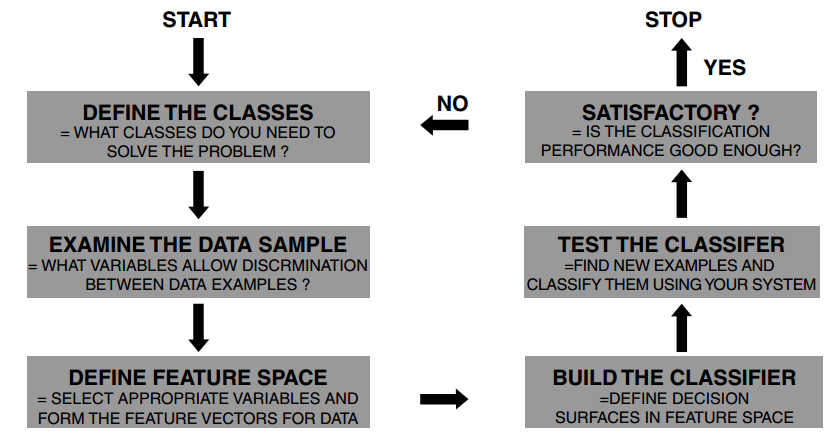
\includegraphics[width=0.80\textwidth]{classifier-design}
        \caption{Diagrama de flujo de los pasos principales en el diseño de un clasificador \parencite{Solomon2011-xz}}
        \label{fig:classifier-design}
    \end{figure}
    

